%%% spell check: aug29 2014
%%%% handouts:  pdfjam --landscape --nup '2x2' ecology1.pdf
%%%% handouts:  pdfjam --landscape ecology1.pdf


%%% PRIOR TO CLASS: have all participants download the class data into
%%% a working directory on their computer; make sure all computers
%%% have a current version of R

%\documentclass[handout]{beamer}
\documentclass[10pt]{beamer}
\usepackage{parskip}
\usepackage{fancyvrb}
\usepackage{graphicx}
\setlength{\parskip}{1.75ex}

\mode<presentation>
{\usetheme{Singapore}
\setbeamercovered{transparent}}

\title{R Minicourse Workshop}

\author{\small Presented to the\\
        Washington State Deptment of Ecology\\
       September 2--3, 2014}

\date{\scriptsize Dr.~Robin Matthews, Institute for Watershed Studies\\
   Dr. Geoffrey Matthews, Computer Science Department\\
   Western Washington University}


\setbeamertemplate{blocks}[rounded][shadow=true]
\setbeamertemplate{footline}{\hspace*{5ex}Part 1 - Sept.~2, 2014 
   \hfill Page \insertframenumber \hspace{0.1ex} of
   \inserttotalframenumber \hspace*{5ex}
   \vspace*{2ex}}

\newcommand{\red}{\color{red}}
\newcommand{\blue}{\color{blue}}
\newcommand{\iwsframe}[2]{
\begin{frame}[fragile]
\frametitle{#1}
\framesubtitle{#2}
}

\begin{document}
\lecture{R Minicourse}{Section 1}
\newcommand{\be}{\begin{enumerate}}
\newcommand{\ee}{\end{enumerate}}
\newcommand{\bi}{\begin{itemize}}
\newcommand{\ei}{\end{itemize}}
\newcommand{\bd}{\begin{description}}
\newcommand{\ed}{\end{description}}


\begin{frame}
\titlepage
\end{frame}

\begin{frame}
\frametitle{Preliminary Schedule}

{\scriptsize
\begin{tabular}{llp{3in}}
{\bf September 2} & & \\\hline
8:30--11:00 & Part 1 & Basics, including importing/exporting data,
writing/running source files, importing/running packages, extracting
information, generating univariate descriptive statistics\\
  & & \\
11:00--12:00 & & Questions/one-on-one instruction\\
  & & \\
12:00--1:00  & & Lunch \\
  & & \\
1:00--3:30 & Part 2 & Plotting, including xy-scatterplots,
boxplots, overlay plots, dual axis plots, and basic/intermediate
formatting\\
  & & \\
3:30--4:30 & & Questions/one-on-one instruction\\
  & \\
{\bf September 3} & &\\\hline
8:30--11:00 & Part 3 & Bivariate analysis, including regression,
correlation, ANOVA; testing assumptions;
transformations, and nonparametric alternatives\\
  & \\
11:00--12:00 & & Questions/one-on-one instruction\\
  & \\
12:00--1:00 & & Lunch \\
  & \\
1:00--3:30 & Part 4 & Ordination, clustering (hierarchical, divisive, pca), association analysis\\
  & \\
3:30--4:30 & & Questions/one-on-one instruction\\
\end{tabular}
}
\end{frame}


\iwsframe{Quick Introduction to R}{A Very Powerful Calculator}

\begin{Verbatim}[commandchars=\\\{\}]
\red 3 + 4*(99 - 2)
\blue[1] 391
\red c(1,2,3) + c(100, 200, 300)
\blue[1] 101 202 303
\red c(1,2,3) * 10
\blue[1] 10 20 30
\red 1:9 + 3
\blue[1]  4  5  6  7  8  9 10 11 12
\red sin(pi)
\blue[1] 1.224606e-16
\end{Verbatim}
\bi
\item My input in {\red red}, R's response in {\blue blue}
\item {\red c} catenates numbers into a {\em vector}
\item Note that floating point arithmetic is always {\em approximate}
\item Can use arrow keys to recall commands
\ei
\end{frame}

\iwsframe{Quick Introduction to R}{Matrix Math}
\begin{columns}
\column{0.5\textwidth}
\begin{Verbatim}[commandchars=\\\{\}]
\red a <- rbind(1:3, 4:6)
\red a
\blue     [,1] [,2] [,3]
\blue[1,]    1    2    3
\blue[2,]    4    5    6
\red b <- cbind(11:13, 14:16)
\red b
\blue     [,1] [,2]
\blue[1,]   11   14
\blue[2,]   12   15
\blue[3,]   13   16
\red a %*% b
\blue     [,1] [,2]
\blue[1,]   74   92
\blue[2,]  182  227
\end{Verbatim}
\column{0.5\textwidth}
\bi
\item We can name mathematical objects with the {\red \tt <-} operator
\vspace{1ex}
\item {\red cbind} binds {\red c}olumns
\vspace{1ex}
\item {\red rbind} binds {\red r}ows\newline
\vspace{1ex}
\item Without the \verb|%*%| operator, multiplication is component-wise:
\ei
\begin{Verbatim}[commandchars=\\\{\}]
\red 1:5
\blue[1] 1 2 3 4 5
\red 5:1
\blue[1] 5 4 3 2 1
\red 1:5 * 5:1
\blue[1] 5 8 9 8 5
\end{Verbatim}
\end{columns}
\end{frame}

\iwsframe{Quick Introduction to R}{Data Frames}


\begin{Verbatim}[commandchars=\\\{\}]
\red mydata <- data.frame(1:12, gl(3,4), rnorm(12), runif(12))
\red names(mydata) <- c("ID", "Group", "X", "Y")
\red mydata
\blue   ID Group           X         Y
\blue1   1     1 -1.14494014 0.4477421
\blue2   2     1  0.78868969 0.1427814
\blue3   3     1  2.06218090 0.5848855
\blue4   4     1 -0.99460233 0.6999962
\blue5   5     2  0.41466492 0.2406326
\blue6   6     2 -0.81099703 0.3214530
\blue7   7     2  0.54504343 0.1111105
\blue8   8     2 -0.65916912 0.3415629
\blue9   9     3 -0.51886246 0.3548058
\blue10 10     3 -0.02180427 0.8345689
\blue11 11     3  0.51281399 0.5886773
\blue12 12     3 -1.58794920 0.8442706
\end{Verbatim}
\end{frame}
\iwsframe{Quick Introduction to R}{More Readable Numbers}
\begin{columns}
\column{0.5\textwidth}
\begin{Verbatim}[commandchars=\\\{\}]
\red options(digits=2)
\red mydata
\blue   ID Group      X    Y
\blue1   1     1 -1.145 0.45
\blue2   2     1  0.789 0.14
\blue3   3     1  2.062 0.58
\blue4   4     1 -0.995 0.70
\blue5   5     2  0.415 0.24
\blue6   6     2 -0.811 0.32
\blue7   7     2  0.545 0.11
\blue8   8     2 -0.659 0.34
\blue9   9     3 -0.519 0.35
\blue10 10     3 -0.022 0.83
\blue11 11     3  0.513 0.59
\blue12 12     3 -1.588 0.84
\end{Verbatim}
\column{0.5\textwidth}
\bi
\item R maintains internal accuracy; this is to
  unclutter the display
\vspace{1ex}
\item FYI - R uses 32-bit floats with double-precision
  arithmetic
  \ei
\end{columns}
\end{frame}
\iwsframe{Quick Introduction to R}{Quick Plotting}
\begin{columns}
\column{0.4\textwidth}
\begin{Verbatim}[commandchars=\\\{\}]
\red mydata
\blue   ID Group      X    Y
\blue1   1     1 -1.145 0.45
\blue2   2     1  0.789 0.14
\blue3   3     1  2.062 0.58
\blue4   4     1 -0.995 0.70
\blue5   5     2  0.415 0.24
\blue6   6     2 -0.811 0.32
\blue7   7     2  0.545 0.11
\blue8   8     2 -0.659 0.34
\blue9   9     3 -0.519 0.35
\blue10 10     3 -0.022 0.83
\blue11 11     3  0.513 0.59
\blue12 12     3 -1.588 0.84
\red plot(mydata)
\end{Verbatim}
\column{0.6\textwidth}
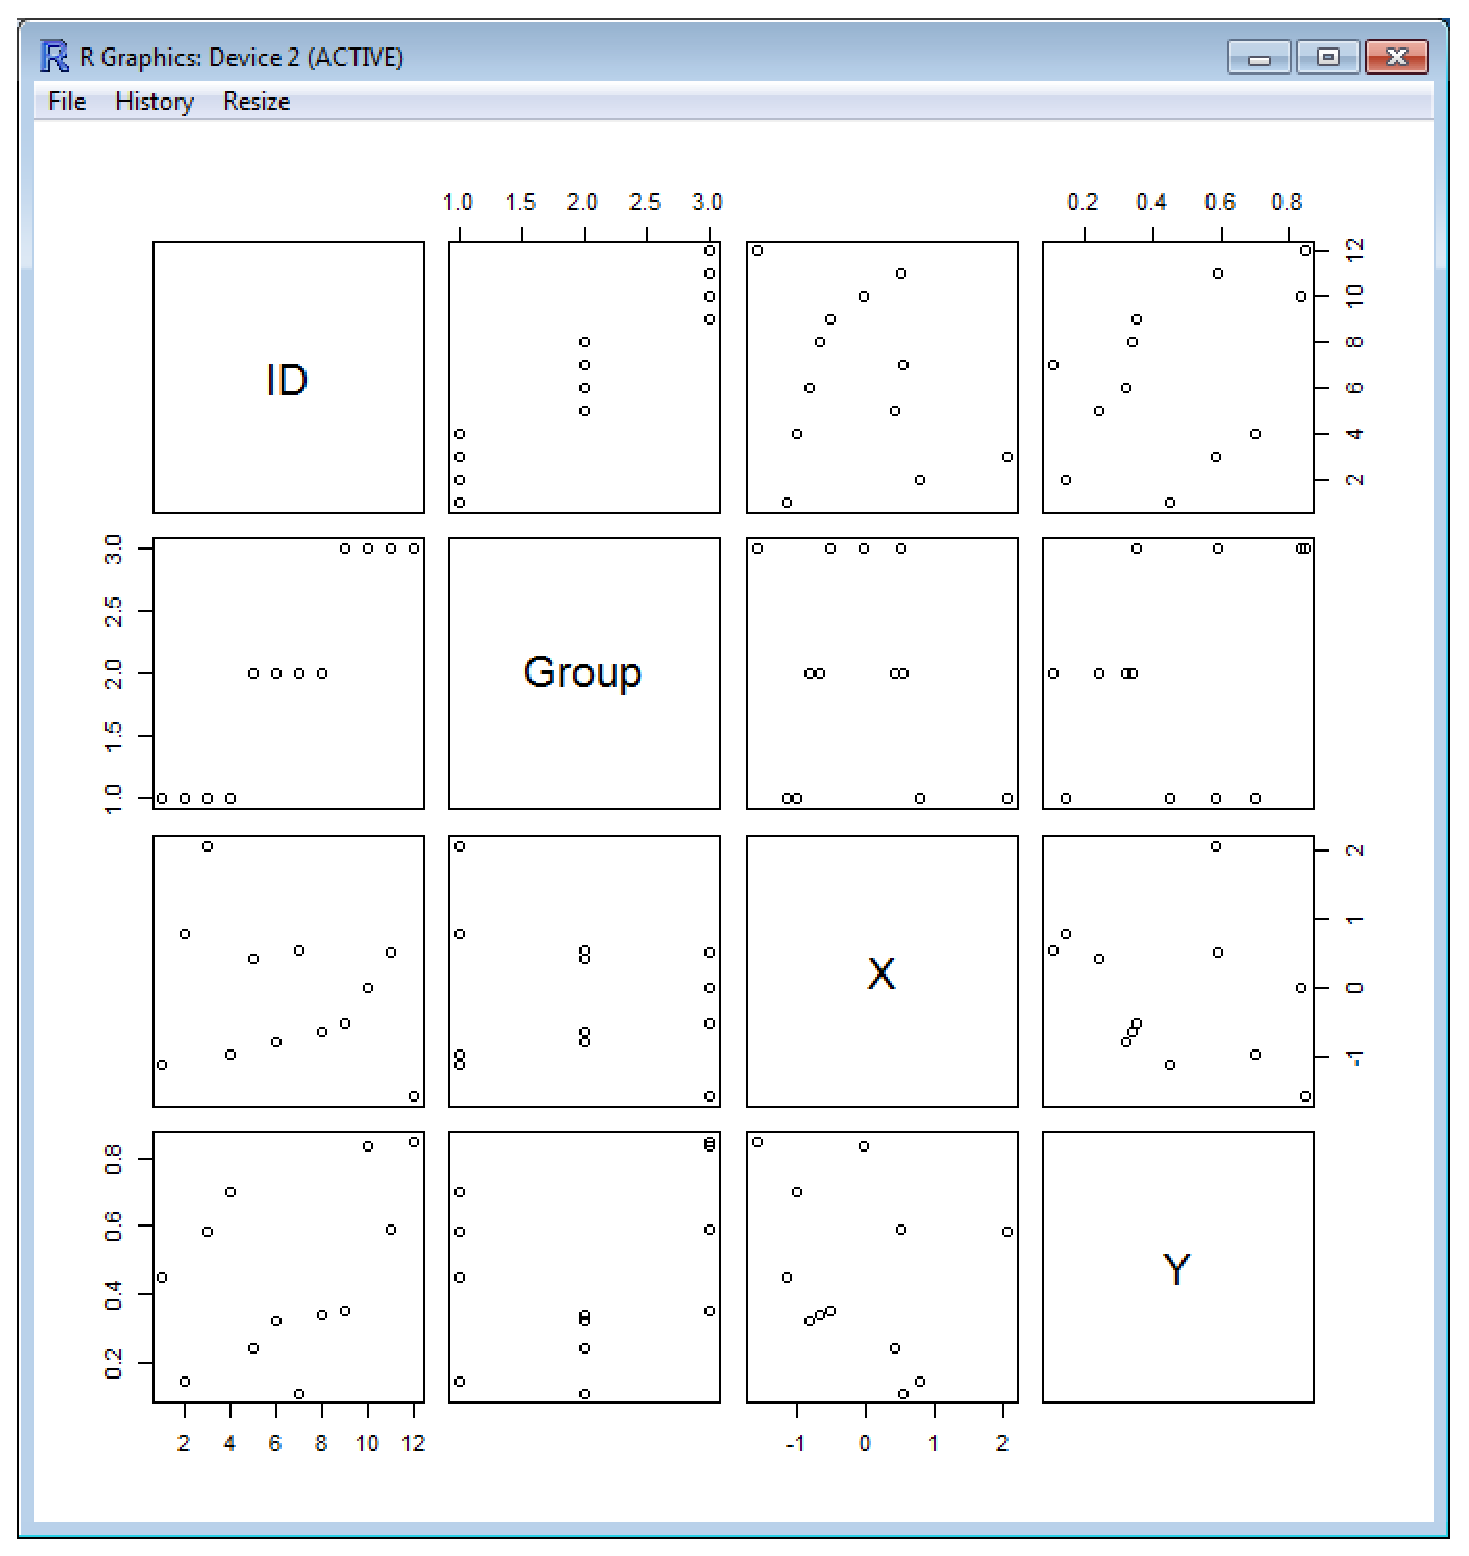
\includegraphics[width=\textwidth]{./screenshots/plotmydata.eps}
\end{columns}
\end{frame}


\begin{frame}[fragile]
\frametitle{Collecting and Entering Data}
\framesubtitle{Quantitative vs.~Categorical Data}

\bi
\item Numerical {\em quantitative} (measured) or {\em categorical}
  (grouped)

\item Categorical information may be further subdivided:
  \bi
  \item Nominal (groups have no order) $\ldots$ red, blue, yellow
  \item Ordinal (groups are ordered) $\ldots$ low, medium, high
  \item Interval (groups are assigned ranges) $\ldots$ 0--1,
    1--10, 10--100
  \item Hierarchical (groups are ``nested'' in the hierarchy)\\
  \ei

\item Quantitative data can be used to create categories (e.g., TP
  $\ge$ 20 $\mu$g/L = high; TP $<$ 20 $\mu$g/L = low)

\item Ordinal and interval data can be ranked for 
  nonparametric tests (e.g., low/med/high = 1/2/3)\\
\ei

\end{frame}


\begin{frame}
\frametitle{Collecting and Entering Data}
\framesubtitle{ASCII Data and Data Set Structure}

\bi
\item Most statistical programs can read {\bf ASCII}$^{\dag}$
  data\\
\hspace*{5ex}{\tiny $^{\dag}$American Standard Code for Information Interchange}

\item Many programs can read Excel files if you follow formatting rules 
	\bi
	\item Fill all cells with numbers or codes ($\Rightarrow$no empty cells!)
	\item Use correct entries for zero (0) and missing data ({\color{red} {\tt R} uses NA})
	\item Columns contain variables; rows contain unique samples
        \item Do not use spaces in categorical entries or variable names
	\item Decide how to handle {\em out of range} data
          (see next slide)
	\item Enter comments and categorical data in a format that will work
	for the statistical program, not just Excel
       \item Be consistent (NA $\ne$ na $\ne$ n/a $\ne$ N/A; RED $\ne$ Red $\ne$ red)\\
        \ei 
\ei
\end{frame}


\begin{frame}
\frametitle{Collecting and Entering Data}
\framesubtitle{Common Data Set Problems - Out of Range Data}

\bi 
\item Out of range data are usually flagged using a nonnumeric
  code\\($<$, $>$, bdl)

\item For statistical purposes you need to decide whether to 
	
	\bi
	\item Omit these data
        \item Change methods to avoid out of range values
	\item Substitute a single value (e.g., one-half the difference
	between zero and the lowest measurable value)
	\item Try to approximate the value using a distribution model
        \item Use ``uncensored'' values (might include negative numbers)
	\ei

\item What you {\em can't} do is enter ``$<$5'' with
  other numeric values because it converts the entire column to a
  categorical variable \\ \ei
\end{frame}


\begin{frame}[fragile]
\frametitle{Collecting and Entering Data}
\framesubtitle{Common Data Set Problems - Unbalanced Data Sets}

\bi
\item A balanced data set has the same number of entries for every
column (no NAs)

\item Multivariate data sets are often unbalanced

	\bi 
	\item Samples can be lost, broken, contaminated; some parameters may
          be measured more frequently than others 
        \ei

\item Many statistical programs will not run on unbalanced data unless
  you specify how to deal with the missing values

\item The command {\color{red} \tt na.rm=T} is used in {\color{red}
  \tt R} to indicate that missing values should be omitted from the
  calculation\footnote{\tiny NOTE: Commands will continue in
    {\color{red} \tt red}; responses in {\color{blue}\tt blue};
    {\color{red} \tt >} and non-essential output will be omitted\\}

{\scriptsize
\color{red}
\verb%x <- c(1,2,3,4,NA)%\\
\verb%mean(x)%\\
\color{blue}
\verb%[1] NA%\\
\color{red}
\verb%mean(x, na.rm=T)%\\
\color{blue}
\verb%[1] 2.5%\\
}

\ei
\end{frame}

\begin{frame}[fragile]
\frametitle{Collecting and Entering Data}
\framesubtitle{Common Data Set Problems - Measurement Units}

\bi
\item Some statistical tests are influenced by measurement units
  (e.g., from mg/L to $\mu$g/L), especially tests based on squared
  variance

\item There is no single solution to this problem, but transformations
  (log, etc.) and rank-based tests are common approaches

{\scriptsize
\color{red}
\verb%a <- c(1000, 2000, 3000, 4000, 5000)%\\
\verb%b <- c(4000, 5000, 6000, 7000, 8000)%\\
\vspace{1ex}
\verb%t.test(a,b)%\\

\vspace{1ex}
\color{blue}
\verb%Welch Two Sample t-test ### edited output%\\
\verb%t = -3, df = 8, p-value = 0.01707%\\

\vspace{2ex}
\color{red}
\verb%kruskal.test(a,b)%\\
\vspace{1ex}
\color{blue}
\verb%Kruskal-Wallis rank sum test ### edited output%\\
\verb%Kruskal-Wallis chi-squared = 4, df = 4, p-value = 0.406%\\
}

\ei
\end{frame}
 
\begin{frame}
\frametitle{Exercise \#1 - Importing/Exporting Data}
\framesubtitle{Institute for Watershed Studies Northwest Lakes Monitoring Data}

{\scriptsize Background information: The Institute for Watershed
  Studies has collected water quality data from more than 65 lakes in
  northwest Washington since 2007 as a public service and to provide
  internships for WWU students.  A subset of the lakes data are
  included in lakes.xlsx.  The data were edited to exclude rows with
  missing values and lakes with more than one sampling location. The
  remaining file contains data from 65 lakes in Whatcom, Skagit,
  Snohomish, and Island Counties\\}
%%% length(unique(site)) - removed NA rows; removed KWAN/TBIRD/SAM1-4

\vspace{2ex}
{\scriptsize
\begin{tabular}{ll} 
\multicolumn{2}{l}{Summary of variables in lakes.xlsx}\\ \hline
site   & Short lake names (no spaces!)\\
month  & Month (separate column)\\
day    & Day (separate column)\\
year   & Year (separate column)\\
chl    & Chlorophyll ($\mu$g/L) - algae biomass\\
do     & Dissolved oxygen (mg/L) - high oxygen levels indicate active photosynthesis\\
temp   & Water temperature (C) - warm lakes often have more algae\\
ph     & pH - measure of lake acidity; indicates high levels of photosynthesis if $>$8\\
cond   & Specific conductance ($\mu$S/cm) - measure of dissolved salts\\
alk    & Alkalinity (mg/L) - measure of lake buffering capacity (resistance to pH change)\\
turb   & Turbidity (NTU) - measure of lake clarity\\
nh3    & Ammonium ($\mu$g-N/L) - algal growth nutrient; Cyanobacteria don't need this\\
tn     & Total persulfate nitrogen ($\mu$g-N/L) - inorganic and organic nitrogen\\
no3    & Nitrate/nitrite ($\mu$g-N/L) - algal growth nutrient; Cyanobacteria don't need this\\
tp     & Total persulfate phosphorus ($\mu$g-P/L) - inorganic and organic phosphorus\\
srp    & Soluble phosphate ($\mu$g-P/L) - growth nutrient for all types of algae\\ \hline
\end{tabular}
}
\end{frame}


\begin{frame}
\frametitle{Exercise \#1, continued}
\bi
\item Open ``lakes.xlsx'' using Excel and examine the data file
   \bi
{\small
   \item The first row contains simple column labels (no spaces)
   \item Columns 1-4 contain site and sampling dates (month, day,
     year)
   \item Columns 5-16 contain {\em uncensored} water
     quality data
   \item Some lakes were sampled only once, while others were sampled
     multiple years and multiple times within a single year
}   \ei
\item Save the file as ``lakes.csv'' in your {\color{red} {\tt
    R}-minicourse} working directory\\ We will use this file for
  examples in the next section

\item Open an {\tt \color{red} R} terminal window (double-click on the
  {\tt \color{red} R icon}) and change the working directory to your
  {\color{red} \tt R-minicourse} directory

\ei
\end{frame}


\begin{frame}[fragile]
\frametitle{Exercise \#1, continued}
\label{example1}
\bi
\item Read the data into {\color{red} \tt R} by
  typing the following commands

{\scriptsize
\color{red}
\verb%lakes <- read.csv("lakes.csv", header=TRUE)%\\

\vspace{1ex}
\verb%### here is a shorter option:%\\
\verb%lakes <- read.csv("lakes.csv", T)%\\

\vspace{1ex}
\verb%### here is a more versatile option that works with other types of files:%\\
\verb%lakes <- read.table("lakes.csv", header=TRUE, sep=",")%\\
}

\item Now attach and summarize the data

{\scriptsize
\color{red}
\verb%attach(lakes);summary(lakes)  ### note two commands on one line%\\   
\verb%### "attach" lets you use variable names during the work session%\\
\verb%### "summary" lists simple descriptive stats and is a good verification tool%\\


\color{blue}
\verb%      site         month             day             year            do %\\       
\verb%REE    : 15   Min.   :1.000   Min.   : 1.00   Min.   :2007   Min.   : 0.500  %\\
\verb%FAZ    : 12   1st Qu.:6.000   1st Qu.:14.00   1st Qu.:2008   1st Qu.: 8.100  %\\
\verb%TER    : 12   Median :7.000   Median :20.00   Median :2010   Median : 8.890  %\\
\verb%BUG    : 11   Mean   :6.741   Mean   :19.17   Mean   :2010   Mean   : 8.903  %\\
\verb%SQA    : 11   3rd Qu.:8.000   3rd Qu.:26.00   3rd Qu.:2012   3rd Qu.:10.000  %\\
\verb%SUN    : 11   Max.   :9.000   Max.   :31.00   Max.   :2013   Max.   :21.500  %\\
\verb%(Other):306                                                                  %\\
}
\vspace{1ex} 
{\tiny \color{black} etc.~for remaining variables; note that the lakes
  are listed in order of the most frequently sampled, not
  alphabetically or in the order they are arranged in the data
  matrix\\} \ei
\end{frame}



\begin{frame}[fragile]
\frametitle{Extracting Information from a Data Matrix}
\bi
\item One of the goals in statistical analysis is to extract
  summary information for specific types of measurements

\item {\color{red} \tt R} has many features to do this $\ldots$ too many to
  cover in this class, but we will look at a few
  examples
\item It helps if you understand a few basic features of a typical
  data matrix

\bi
\item A data matrix contains {\color{blue}$p$}
attributes measured on {\color{blue}$N$} samples

\item A matrix denoted {\color{blue} {\bf A}$_{N \times p}$} has
  {\color{blue}$N$} rows and {\color{blue}$p$} columns

\item Individual elements are identified as {\color{blue}$a_{i,j}$}
where {\color{blue}$i$} is the row and {\color{blue}$j$} is the column
\ei

\ei
\end{frame}


\begin{frame}
\frametitle{Simple Data Matrix Example}

\bi
\item This matrix contains four columns, but only the second two
  columns contain measured data (temperature and oxygen). The first
  two columns contain categorical information about the sampling
  location

{\small
\begin{center}
\begin{tabular}{|l|c|c|c|c|} \hline
           & column 1 & column 2 & column 3 & column 4 \\ \cline{2-5}
header row & Location & Type   & Temperature	& Oxygen \\ \hline
row 1      & A        & stream & 10.1		& 12.5 \\  \hline
row 2      & A        & lake   & 7.2 		& 4.2 \\ \hline
row 3      & B        & stream & 10.5		& 12.3\\ \hline
row 4      & B        & lake   & 6.1 		& 0.1 \\ \hline
\end{tabular}
\end{center}
}

\item The data matrix, therefore, has four rows and two column
  ({\color{blue}{\bf X}$_{4 \times 2}$})
	
\item Element {\color{blue}$x_{1,1}$} is 10.1, element {\color{blue}$x_{4,2}$}
is 0.1, etc.

\item The {\color{red} \tt lakes.csv} file contains 378 rows
  and 16 columns, but the first four columns contain site, month, day,
  year.  The water quality data are in columns 5--16
\ei
\end{frame}


\begin{frame}[fragile]
\frametitle{Calculating Simple Descriptive Statistics}

Here are some examples for using {\color{red} \tt R} to calculate
simple descriptive statistics for a single variable (conductivity).
Note that the last three examples are slightly more complicated

{\scriptsize
\begin{tabular}{lll}
                    &                                & Conductivity example\\
Function            & {\color{red} \tt R} syntax     & from lakes.csv\\\hline
Mean                & {\color{red} \tt mean(X)}      & {\color{red} \tt mean(cond)}\\
Median              & {\color{red} \tt median(X)}    & {\color{red} \tt median(cond)}\\ 
Minimum             & {\color{red} \tt min(x)}       & {\color{red} \tt min(cond)}\\
Maximum             & {\color{red} \tt max(X)}       & {\color{red} \tt max(cond)}\\
Number of values    & {\color{red} \tt length(X)}    & {\color{red} \tt length(cond)}\\
Trimmed mean        & {\color{red} \tt mean(X, trim=0.05)} & {\color{red} \tt mean(cond, trim=0.05)}\\
Sample variance     & {\color{red} \tt var(X)}                  & {\color{red} \tt var(cond)} \\
Standard deviation  & {\color{red} \tt sd(X)}                   & {\color{red} \tt sd(cond)}\\
                    &                                           & \\
Geometric mean      & {\color{red} \tt $10^{(\tt mean(log10(X)))}$} & {\color{red} $10^{(\tt mean(log10(cond)))}$}\\
                    &                                           & \\
Standard error of the mean & {\color{red} \tt sqrt(var(X)/length(X))} & {\color{red} \tt sqrt(var(cond)/length(cond))}\\
                    &                                           & \\
95\% conf.~interval & {\color{red} \tt t.test(X)}               & {\color{red} \tt t.test(cond)}\\\hline
\end{tabular}
}

\end{frame}

\begin{frame}[fragile]
\frametitle{Equivalent Statements in {\color{red} \tt R}}

\bi
\item {\color{red} \tt R} is a very sophisticated statistics program
  that includes shortcuts and syntax variations.  Each of the
  following statements will calculate mean conductivity for all sites
  and dates combined (n=378)

\bi
\item {\color{red} \verb%mean(cond)%} - This statement works if
  you attached the variable names (first row) after reading the data


\item {\color{red} \verb%mean(lakes$cond)%} - 
This statement will work with or without attaching the variable names,
but you still need {\color{red} \tt header=TRUE}

\item {\color{red} \verb%mean(lakes[c(1:378), 8])%} - This statement
  works for any data table by specifying the exact rows (1:378) and
  column (8) that contain the conductivity data

   
If there {\em is} a header line, you need {\color{red} \tt
  header=TRUE} because it tells {\color{red} \tt R} that the first row
doesn't contain data

\ei
\ei
\end{frame}

\begin{frame}[fragile]
\frametitle{Selecting Specific Subsets from the Data}

\bi
\item {\color{red} \tt R} uses simple arithmetic operators to select
  specific rows or columns

{\scriptsize
\begin{tabular}{lclc}
Selection    & {\color{red} \tt R Syntax}  & Selection                & {\color{red} \tt R Syntax}\\ \hline
Equal        & {\color{red} \tt == }       & Not equal                & {\color{red} \tt !=}\\
Less than    & {\color{red} \tt < }        & Less than or equal       & {\color{red} \tt <=}\\
Greater than & {\color{red} \tt > }        & Greater than or equal    & {\color{red} \tt >=}\\
And (all must be true) & {\color{red} \tt \&}  & Or (any can be true)  & {\color{red} \tt |}\\\hline
\end{tabular}
}

\item When using {\color{red} \tt R} selection statements, 
  select rows first, then columns, enclosing the selection inside
  brackets.  To select categorical values (e.g., site), enclose
  the value in quotes

{\scriptsize \color{red}
\verb%mean(cond[year==2013])  ### mean 2013 conductivity, all sites%\\

\vspace{2ex}
\verb%mean(cond[year==2013 & site !="WIS"])%\\
\verb%### mean 2013 conductivity for all sites except Wiser Lake%\\

\vspace{2ex}
\verb%mean(cond[site=="WIS"])     ### mean 2007-2013 conductivity, Wiser Lake%\\
\verb%mean([lakes[c(369:378), 8]) ### mean 2007-2013 conductivity, Wiser Lake%\\
}
\ei

\end{frame}



\begin{frame}[fragile]
\frametitle{Descriptive Statistics for Groups of Data}

\bi
\item You can generate results for groups of variables using 
  {\color{red} \tt summary(lakes)} (see page
    \pageref{example1})

\item Another option is to use grouping functions like {\color{red}
  \tt tapply}, {\color{red} \tt lapply}, {\color{red} \tt sapply},
  {\color{red} \tt by}

{\color{red} \scriptsize
\verb%round(sapply(lakes[c(1:378), c(5:16)], mean), 1)%\\ 

\color{blue}
\verb%   do  temp    ph  cond   chl   alk  turb   nh3    tn   no3    tp   srp%\\
\verb%  8.9  18.1   7.6 118.0  13.8  35.0   3.9  18.6 684.5 103.5  31.8   7.1%\\
\vspace{1ex}
\verb%### I selected all rows, but only columns 5-16 ... why?%\\
\verb%### here is a shorter way to select all rows: lakes[, c(5:16)]%\\


\vspace{3ex}
\color{red} 
\verb%by(cond, site, summary)%\\
\color{blue}
\verb%site: ARM%\\
\verb%   Min. 1st Qu.  Median    Mean 3rd Qu.    Max. %\\
\verb%  53.00   54.50   58.05   59.28   62.82   68.00 %\\
\verb%------------------------------------------------------------ %\\
\verb%site: BAGL%\\
\verb%   Min. 1st Qu.  Median    Mean 3rd Qu.    Max. %\\
\verb%  10.00   11.00   12.00   12.12   12.60   15.00 %\\
\verb%------------------------------------------------------------ %\\
\verb%### (etc for remaining lakes) %\\
}

\ei
\end{frame}




\begin{frame}[fragile]
\frametitle{Writing Simple Functions}

\bi
\item One of the features of {\color{red} \tt R} is that is it
programmable. You can create simple functions or entire custom packages

\item Writing a simple function to calculate Standard Error of the Mean

{\color{red} \scriptsize
\verb%SE <- function(x) sqrt(var(x)/length(x))%\\
\verb%SE(cond)%\\
\color{blue}
\vspace{1ex}
\verb%4.611665%\\
\color{red}
\vspace{1ex}
\verb%round(SE(cond), 1)%\\
\color{blue}
\verb%4.6%\\
}

\item  Writing a more complex function to estimate 95\% confidence interval

{\color{red} \scriptsize
\verb%ci95 <- function(x)   {  %\\   
\verb%t.value <- qt(0.975, length(x)-1)%\\
\verb%standard.error <- SE(x)%\\
\verb%ci <- t.value * standard.error%\\
\verb%cat("95 CI = ", round(mean(x) -ci, 1), "to ", round(mean(x) +ci, 1), "\n")  }%\\

\vspace{3ex}

\verb%ci95(cond)%\\
\color{blue}
\verb%95 CI =  109 to  127.1%\\
}
\ei
\end{frame}

\begin{frame}[fragile]
\frametitle{Exercise \#2 - Modifying Simple Functions}
\bi
\item Modify the {\color{red} \tt SE} function to calculate the standard error of
  the mean for total phosphorus (tp)\\
  (Answer = 3.2 $\mu$g-P/L)

{\scriptsize
{\em Discussion:} The IWS data are uncensored, so there are
negative values in the total phosphorus results ({\color{red} \tt min}
= -9.5 $\mu$g/L).  How does this influence variance-based statistics
like the standard error?\\}

\item Modify the {\color{red} \tt SE} function to select 
  lakes with total phosphorus $\ge$3.2 $\mu$g/L (IWS detection limit)\\
Answer = 3.5 $\mu$g/L

\item {\em Optional:} Modify {\color{red} \tt ci95} to calculate the
  95\% confidence interval for total phosphorus in lakes with
  conductivities $\ge$100 $\mu$S\\ Answer: 95 CI = 37.3 to 63.8

\ei
\end{frame}


\begin{frame}[fragile]
\frametitle{Saving Output to a Data Matrix}
\label{savingoutput}

\bi
\item We saw that the {\tt \color{red} tapply} command can be used to repeat
  $\Rightarrow$simple functions

{\scriptsize \color{red} 
\verb%> round(tapply(cond, site, mean),1)%\\
\color{blue} 
\verb%  ARM  BAGL  BAGU   BAK   BEA  BEAR   BIG   BUG   CAI   CAM   CAV   CAY   CED%\\
\verb%  59.3  12.1  12.9  33.6 106.5   5.8  89.2 139.9  59.4 261.3  31.2  19.0  55.0%\\
\color{black}
(etc.)
}

\item We can create a temporary object that contains the results:
{\scriptsize \color{red}
\verb%sitemean <- round(tapply(cond, site, mean),1)%
}

\item Here is how to create additional summary statistics, then
  ``stack'' the results into a new data matrix using {\color{red} \tt
  cbind}:

{\scriptsize \color{red}
\verb%sitemed  <- round(tapply(cond, site, median),1)%\\
\verb%sitemin  <- round(tapply(cond, site, min),1)%\\
\verb%sitemax  <- round(tapply(cond, site, max),1)%\\
\verb%siteN    <- tapply(cond, site, length)%\\
\vspace{1ex}
\verb%summary.stats <- cbind(sitemin, sitemean, sitemed, sitemax, siteN)%\\
}

\ei

\end{frame}

\begin{frame}[fragile]
\frametitle{Saving Output to a Data Matrix, continued}

\bi
\item This is a more advanced example, following the approach on page \pageref{savingoutput}

\item The objects are stacked into {\color{red} \tt summary.stats}
  using {\color{red} \tt cbind}, then made into a {\color{red} \tt
    data.frame} that includes site names ({\color{red} \tt
    unique(site)})
 
\item The {\color{red} \tt names} function is used to add descriptive
  names to the final data matrix, which is saved using the
  {\color{red} \tt write.table} function

{\scriptsize \color{red}
\verb%lakes <- read.table("lakes.csv", T, sep=",")%\\
\verb%attach(lakes)%\\

\verb%sitemean <- round(tapply(cond, site, mean),1)%\\
\verb%sitemed  <- round(tapply(cond, site, median),1)%\\
\verb%sitemin  <- round(tapply(cond, site, min),1)%\\
\verb%sitemax  <- round(tapply(cond, site, max),1)%\\
\verb%siteN    <- tapply(cond, site, length)%\\
\verb%siteID <- unique(site)%\\

\vspace{1ex}
\verb%summary.stats <- cbind(sitemin, sitemean, sitemed, sitemax, siteN)%\\

\vspace{1ex}
\verb%cond.stats <- data.frame(siteID, summary.stats)%
\verb%names(cond.stats) <- c("Site", "Min", "Mean", "Median", "Max", "Count")%\\

\vspace{1ex}
\verb%write.table(cond.stats, "conductivity.csv",%\\ 
\verb%      quote=F, row.names=F, col.names=T, sep=",")%\\
}

\ei

\end{frame}


\begin{frame}[fragile]
\frametitle{Writing/Running Source Files}


\bi
\item Most {\color{red} \tt R} users do {\em not} type long sequences
  of commands in the terminal window.  

\item Instead, we create ASCII text files containing the {\color{red}
  \tt R} commands

By convention, {\color{red} \tt R} source files use the extension
{\color{red} \tt .R} or {\color{red} \tt .r}, but Windows can make it
hard to save files with this extension

Fortunately, {\color{red} \tt R} also reads source files  with {\color{red} \tt
  .txt} extensions


\item To create a simple source file, open Wordpad or any ASCII
  editor, type the {\color{red} \tt R} syntax below, then save the
  file as {\color{red} \tt simplelake.txt} in your minicourse folder

{\scriptsize \color{red}
\verb%lakes <- read.table("lakes.csv", T, sep=",")%\\
\verb%attach(lakes)%\\
\verb%summary(lakes)%\\
}

\ei

\end{frame}



\begin{frame}[fragile]
\frametitle{Writing/Running Source Files, continued}

\bi
\item Switch to the {\color{red} \tt R} terminal window and type

{\scriptsize \color{red}
\verb%source("simplelake.txt")%\\
}

\vspace{1ex}

$\Rightarrow$Make sure you changed the working directory to your
minicourse folder and saved the source file to that folder

\item If you did everything correctly, you should see nothing but the
  wedge-shaped start of line symbol ({\color{red} \tt >}) because
  {\color{red} \tt R} doesn't automatically print all output

\item Re-open {\color{red} \tt simplelake.txt}, edit the last line
  to include a {\color{red} \tt print} statement, save file, then source the file

{\scriptsize \color{red}
\verb%lakes <- read.table("lakes.csv", T, sep=",")%\\
\verb%attach(lakes)%\\
\verb%print(summary(lakes))%\\
}

\item You should get a statistical summary for {\color{red} \tt lakes.csv} \ei

\end{frame}



\begin{frame}[fragile]
\frametitle{Questions/One-on-One Instruction}

\bi
\item This portion of the minicourse is designed for personalized 
  instruction, so can proceed at your own pace

\item Novice {\color{red} \tt R}-users should review the examples and
  try to generate simple descriptive statistics for a different water
  quality variable (e.g., temperature)

\item Intermediate and advanced {\color{red} \tt R}-users can set up
  source files and work on their own data sets

\item Each section of this minicourse includes an edited source file
  that can be used to duplicate the more complex examples.  The files
  are posted on the IWS web site (www.wwu.edu/iws)

{\scriptsize
\begin{center}
\begin{tabular}{ll}
\multicolumn{2}{c}{{\color{red} \tt R Source Files}}\\\hline
Parts 1 -- 4:             & ecology1.r -- ecology4.r\\
White River case study    & whiteriver.r\\
PCA clustering case study & PCAclustering.r\\ \hline
\end{tabular}
\end{center}
}
\ei

\end{frame}

\iwsframe{Advanced Topics}{R and Dates}

\bi
{\scriptsize
\item Year, month, and day can be converted  with {\tt \red ISOdate} or {\tt \red chron} (discussed in Part 2)
\item Strings of the form ``2012/05/12'' can be converted with {\tt\red strptime}
\item If your dates are factors, convert them first with {\tt \red as.character} 
or create them with {\tt \red stringsAsFactors=FALSE}
\item Resulting objects can be used to plot on the horizontal axis\\
}
\ei

\scriptsize
\begin{Verbatim}[commandchars=\\\{\}]
\red lake.dates <- ISOdate(lakes$year, lakes$month, lakes$day)
\red lake.dates[1]
\blue[1] "2009-08-31 12:00:00 GMT"
\red lake.dates[1] + 1
\blue[1] "2009-08-31 12:00:01 GMT"
\red lake.dates[1] + 24*60*60
\blue[1] "2009-09-01 12:00:00 GMT"
\red strptime("2012/5/12", format="%Y/%m/%d")
\blue[1] "2012-05-12 PDT"
\red strptime("12/5/12", format="%y/%m/%d")
\blue[1] "2012-05-12 PDT"
\red strptime("2012/5/12 13:30:02" , format="%Y/%m/%d %H:%M:%S")
\blue[1] "2012-05-12 13:30:02 PDT"
\red datestrings <- c("2012/5/1", "2015/2/22", "2011/12/25")
\red strptime(datestrings, format="%Y/%m/%d")
\blue[1] "2012-05-01 PDT" "2015-02-22 PST" "2011-12-25 PST"
\end{Verbatim}

\end{frame}

\begin{frame}
\frametitle{Supplemental References}

\bi
\item Crawley, Michael J.  2013.  The R Book.  John Wiley \& Sons. ISBN 978-0-470-97392-9

\item Dalgaard, Peter.  2008.  Introductory Statistics with R, 2nd
  Edition.  Springer. ISBN 978-0-387-79053-4

\item Lander, Jared P.  2014.  R for Everyone, Advanced Analytics and Graphics.  Addison Wesley Data \& Analytics Series,  ISBN 978-0-321-88803-7

\item Teetor, Paul. 2011.  The R Cookbook.  O'Reilly Publishers. ISBN
  978-0-596-880915-7

\ei
\end{frame}

\end{document}
\end



%%  LocalWords:  Minicourse llp xy scatterplots pca catenates rbind
%%  LocalWords:  cbind olumns ows mydata gl rnorm runif unclutter TP
%%  LocalWords:  na nonnumeric bdl NAs xlsx chl ph cond alk turb nh
%%  LocalWords:  persulfate tp srp minicourse Teetor lll sd sqrt conf
%%  LocalWords:  lclc lapply sapply ci txt Wordpad simplelake ISOdate
%%  LocalWords:  strptime datestrings
